%==============================================================================
%  Geometry-resolved characterization of a dual-detector MA-XRF scanner
%  A0 portrait conference poster, two columns.
%
%  ONE PAGE, VERIFIED BY COMPILE (pdfLaTeX, MiKTeX 26.5, 2026-08-24): both
%  columns end at about 105 cm from the top of the 118.9 cm sheet, i.e. with
%  about 11 cm of spare column height each.  Column breaks are forced:
%      column 1   idea (text beside the schematic), two-stage decomposition
%                 (hero, panels side by side), canvas topography
%      column 2   instrument, learned fusion, positioning, take-home box,
%                 acknowledgements
%  The 11 cm of slack is room for text edits; it is not a reason to enlarge
%  the figures, which are already true-size.
%
%  IF IT STILL RUNS LONG, in this order:
%    1. delete the block marked OPTIONAL BLOCK (positioning error budget,
%       column 2) -- POSTER_PLAN.md ranks it last and calls it filler
%    2. re-render the figures narrower and place them at a fixed width
%       (see below)
%
%  FIGURES ARE TRUE-SIZE: they were rendered at exactly \columnwidth, 380 mm
%  (the schematic at 210 mm, so it sits beside its paragraph), so
%  width=\columnwidth is a scale factor of 1 and the axis labels keep the
%  point size they were drawn at.  Re-render with
%      python scripts/18_poster_figures.py --width-mm 380 \
%          --width-override idea=210 --hero-panels side \
%          --positioning-aspect 0.34 --out-dir poster/figures
%      rm poster/figures/*.png
%  and change --width-mm only together with the column geometry in the class.
%
%  Class: Hylangtechposter.  A stand-in ships in this folder so the project
%  compiles as uploaded; see README.md for swapping in the original.
%==============================================================================
\documentclass[portrait]{Hylangtechposter}

% ---- typeface ----------------------------------------------------------------
% Latin Modern everywhere: the class loads lmodern for the text, and the
% figures are drawn in Latin Modern Roman too (scripts/18_poster_figures.py
% registers the OTF files from the MiKTeX tree), so text and figures are one
% face.

% ---- logos -------------------------------------------------------------------
% The three author affiliations that have a logo sit in the header between
% the two rules (IDArtScience has none).  figures/logo_*.png are the files
% from the poster folder trimmed to their ink (scratchpad crop_logos.py);
% Vinca and the Palace keep their navy ground as a badge.  Every logo is
% raised to its vertical centre so the row aligns on the middle, not on the
% baseline.  Ars Mensurae is a 41 px wordmark, so it is kept small.
\newcommand{\logobox}[2]{\raisebox{-0.5\height}{\includegraphics[height=#1]{#2}}}
\renewcommand{\headerlogos}{%
  \logobox{5cm}{figures/logo_etf.png}\hfill
  \logobox{5cm}{figures/logo_vinca.png}\hfill
  \logobox{2.4cm}{figures/logo_arsmensurae.png}}

% Keep each column what the layout says it is: no vertical stretching of the
% glue between blocks, and no automatic balancing of the last column.
\raggedcolumns

% Width of the schematic beside the opening paragraph.  It must match the
% --width-override idea=... the figure was rendered at.
\newlength{\schematicwidth}
\setlength{\schematicwidth}{21cm}

\begin{document}

\printheader

\begin{center}

%% TITLE
\textbf{\bf\veryHuge\color{posterblue}Geometry-resolved characterization of a
dual-detector MA-XRF scanner \\[1.0cm]}

%% AUTHORS
\huge
Dimitrije Pe\v{s}i\'{c}\textsuperscript{1} ~
Janko Vukobratovi\'{c}\textsuperscript{1} ~
Aleksandra Stojanovi\'{c}\textsuperscript{1} ~
Giulia Ristori\textsuperscript{2} \\[0.2cm]
Stefano Ridolfi\textsuperscript{3} ~
Maja Gaji\'{c}-Kva\v{s}\v{c}ev\textsuperscript{4} ~
Goran Kva\v{s}\v{c}ev\textsuperscript{1} \\[0.35cm]

\Large
\textsuperscript{1}School of Electrical Engineering, University of Belgrade \quad
\textsuperscript{2}Ars Mensurae, Rome \\[0.15cm]
\textsuperscript{3}IDArtScience Srl, Rome \quad
\textsuperscript{4}VINARH Center, Vin\v{c}a Institute of Nuclear Sciences

\end{center}

\vspace{1cm}

% a0poster's ladder: \large is 29.86 pt, the 28-32 pt body size POSTER_PLAN.md
% section 4 asks for.
\large

\begin{multicols}{2}

\color{black}

%==============================================================================
%  COLUMN 1
%==============================================================================
\section*{One tilted scan separates detector from geometry}

% Paragraph on the left, schematic on the right: at 38 cm a full-width
% schematic would be 24 cm tall for six shapes.
\noindent
\begin{minipage}[c]{\dimexpr\columnwidth-\schematicwidth-1.2cm\relax}
The two heads see the same spot from opposite take-off angles, so their
count ratio $R$ = upper head / lower head mixes a detector part with a
geometric part. Tilting the canvas moves only the geometric one: a second
scan separates them, with no standards and no extra hardware.
\end{minipage}\hfill
\begin{minipage}[c]{\schematicwidth}
\centering
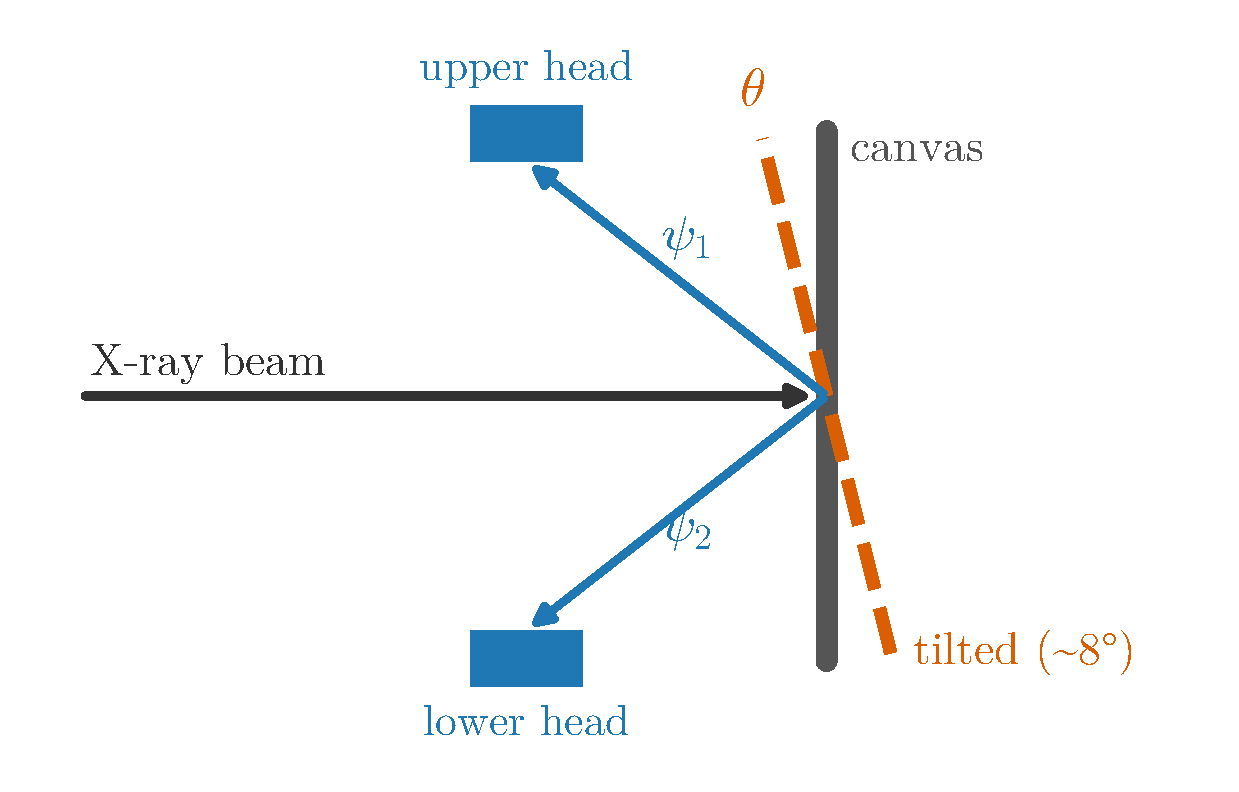
\includegraphics[width=\schematicwidth]{figures/block1_idea_schematic.pdf}
\captionof{figure}{Tilting moves the geometric term only.}
\end{minipage}
\vspace{0.3cm}

%------------------------------------------------------------------------------
\section*{The two heads differ sixfold, and a physical model explains it}

Stage 1 fits the frontal curve with a three-parameter detector model; stage 2
fits the tilt shift with a thick-sample model whose take-off angles move
antisymmetrically with the tilt.

\begin{itemize}
\item $R$ falls from \textbf{5.8} at Ca~K$\alpha$ to \textbf{0.63} at
  Pb~L$\gamma$: a sixfold different signal from the same pigment.
\item Fitted absorber \textbf{973 $\pm$ 2~$\mu$m} Be-equivalent,
  80--120$\times$ any entrance window: extra air path, not a window.
\item The tilt shift decays monotonically; $s = 0.53 \pm 0.10$~deg/deg, and a
  model-free Gaussian-process fit agrees within 1.1$\sigma$.
\end{itemize}

\begin{center}\vspace{0.2cm}
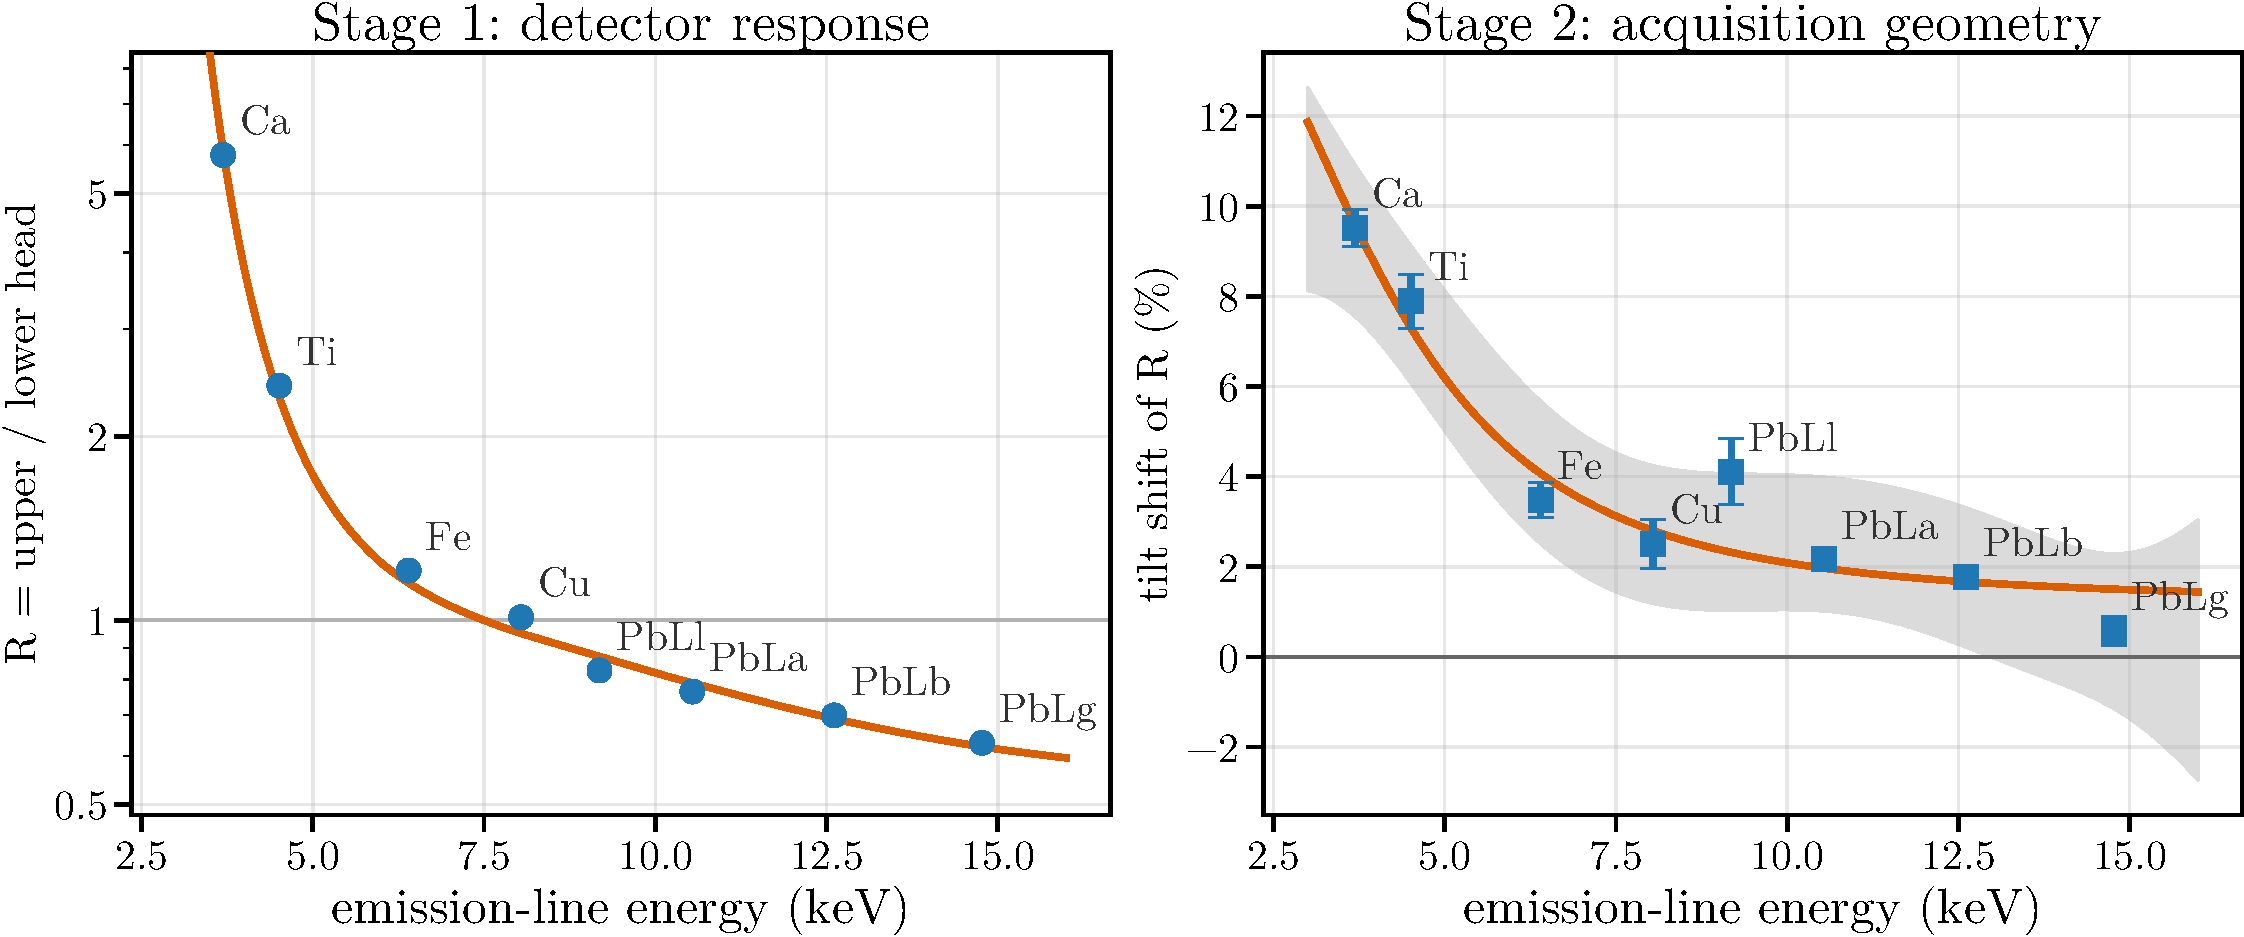
\includegraphics[width=\columnwidth]{figures/block3_hero_geometry_fit.pdf}
\captionof{figure}{Points: measured on the registered overlap. Line: the
physical model of each stage. Band: model-free GP fit, 2$\sigma$.}
\end{center}\vspace{0.2cm}

%------------------------------------------------------------------------------
\section*{The discarded difference is also a relief map}

Inverted through the measured tilt response, the per-pixel ratio residuals
become repeated measurements of local surface slope: cross-scan $r = 0.73$,
RMS $\approx 12^{\circ}$, $\chi^2/\mathrm{dof} = 0.85$, and 88~\% of pixels
consistent with pure geometry: a relief map from one scan.

\begin{center}\vspace{0.2cm}
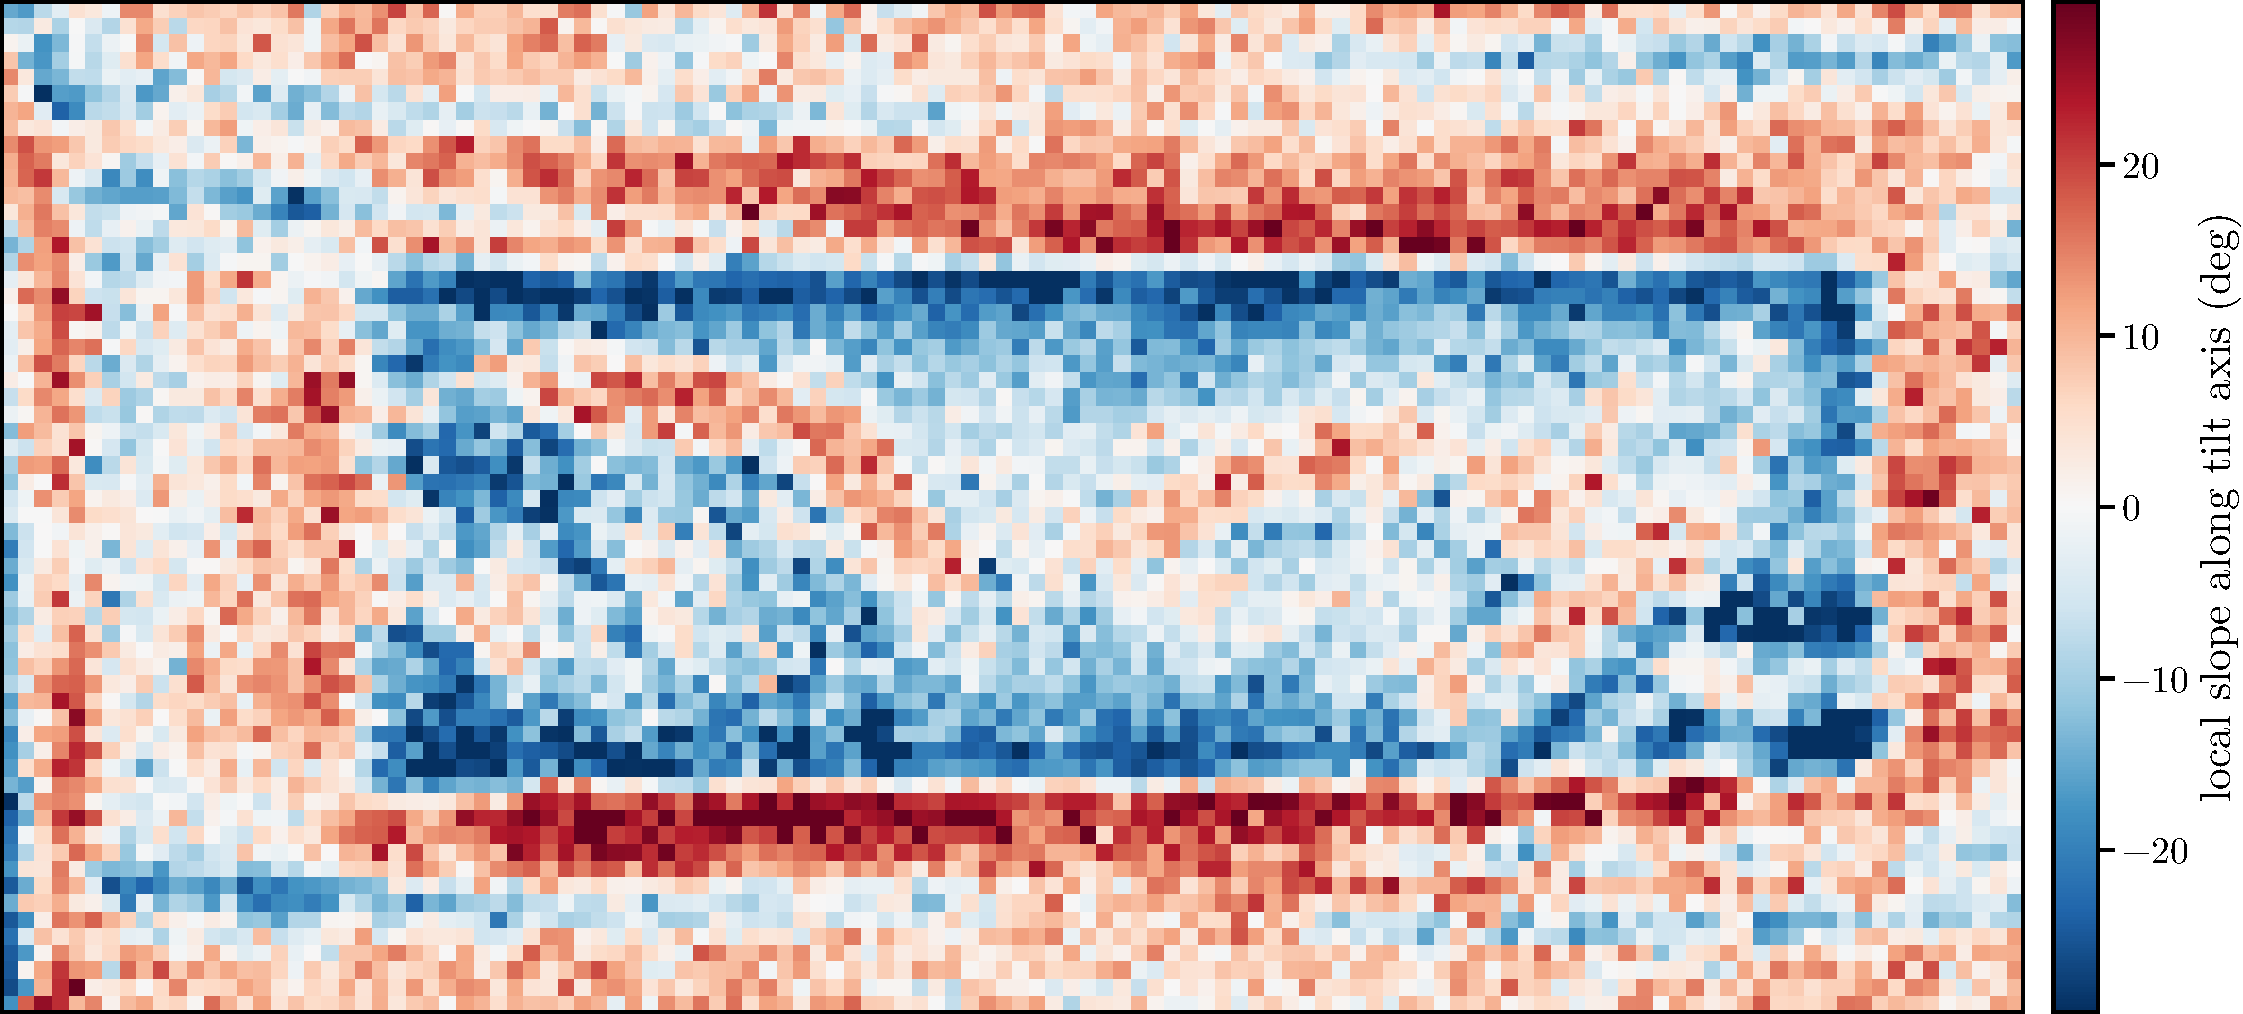
\includegraphics[width=\columnwidth]{figures/block5_canvas_topography.pdf}
\captionof{figure}{Local surface slope along the tilt axis, from one scan.
Detector disagreement measures relief.}
\end{center}

\columnbreak

%==============================================================================
%  COLUMN 2
%==============================================================================
\section*{Two detectors, three scans, 7\,200 pixels}

Ars Mensurae MA-XRF scanner, two Amptek X-123SDD heads, 40~kV / 50~$\mu$A.
Mock-up canvas, $60 \times 120$ pixels, 3.0~s dwell. Two frontal scans seven
days apart set the repeatability baseline; a third is tilted forward by
$\leq 8^{\circ}$. Ratios use the registered overlap (affine, NCC 0.965);
full-frame ratios carry a field-of-view artifact that can flip the shift's
sign.

%------------------------------------------------------------------------------
\section*{Learned fusion beats summing by 10--18~\% SNR}

The two channels are conditionally independent Poisson views of the same
spot, so Noise2Noise training needs no clean target. A 1D U-Net with loss
weights from the measured $R(E)$ gains \textbf{+17.7~\% mean SNR} over
summing on held-out pixels; classical weighting gives +0.9~\%.

\begin{itemize}
\item Six of eight lines gain: Pb~L$\ell$ +69~\%, Pb~L$\gamma$ +33~\%,
  Fe +28~\%, Cu +17~\%.
\item An unweighted loss gives $-0.1$~\%: the gain is the measured variance
  structure, not the architecture. In acquisition time it is worth 39~\%
  longer dwell.
\end{itemize}

\begin{center}\vspace{0.2cm}
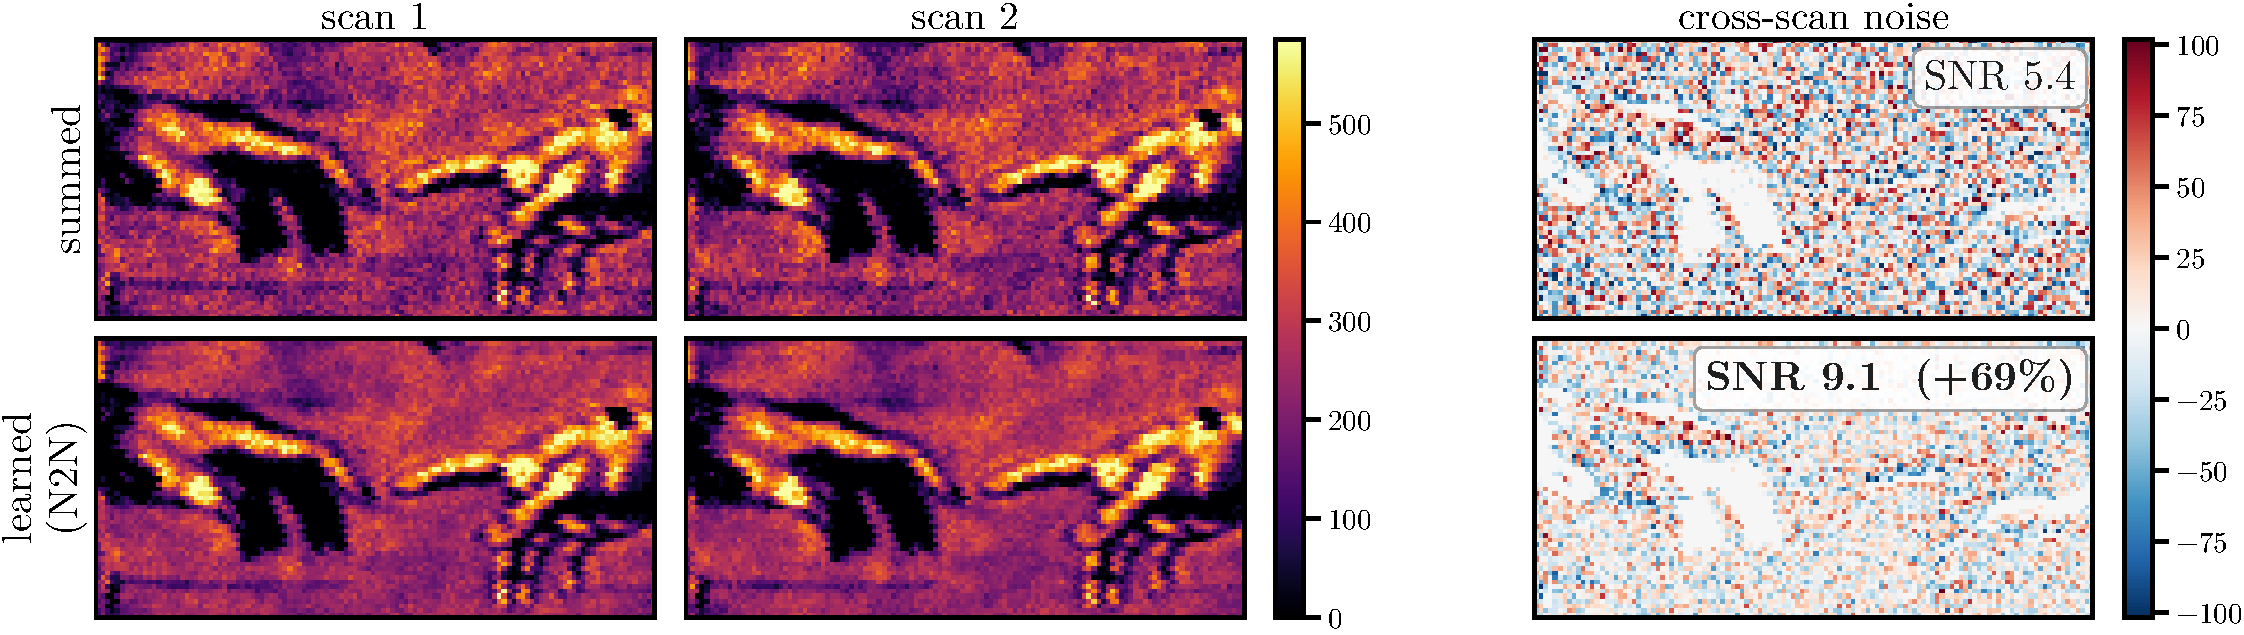
\includegraphics[width=\columnwidth]{figures/block4_fusion_pbll.pdf}
\captionof{figure}{Pb~L$\ell$ on pixels the network never saw: same signal,
calmer noise. Maps in net counts; right, the cross-scan difference.}
\end{center}\vspace{0.2cm}

%%%%%%%%%%%%%%%%%%%%%%%%%%%%%%%%%%%%%%%%%%%%%%%%%%%%%%%%%%%%%%%%%%%%%%%%%%%%%%%
%%% OPTIONAL BLOCK -- first thing to delete if the poster runs long (~22 cm).
%%% POSTER_PLAN.md ranks this last and calls it filler.
%%%%%%%%%%%%%%%%%%%%%%%%%%%%%%%%%%%%%%%%%%%%%%%%%%%%%%%%%%%%%%%%%%%%%%%%%%%%%%%
\section*{One degree of mounting error moves the maps}

One degree of mounting error moves the element maps by up to \textbf{0.63
percentage points} (Ca +0.50~\%/$^{\circ}$, Ti +0.45~\%/$^{\circ}$,
Pb~L$\beta$ $-0.13$~\%/$^{\circ}$), in the energy order the model predicts.
These are lower bounds.

\begin{center}\vspace{0.2cm}
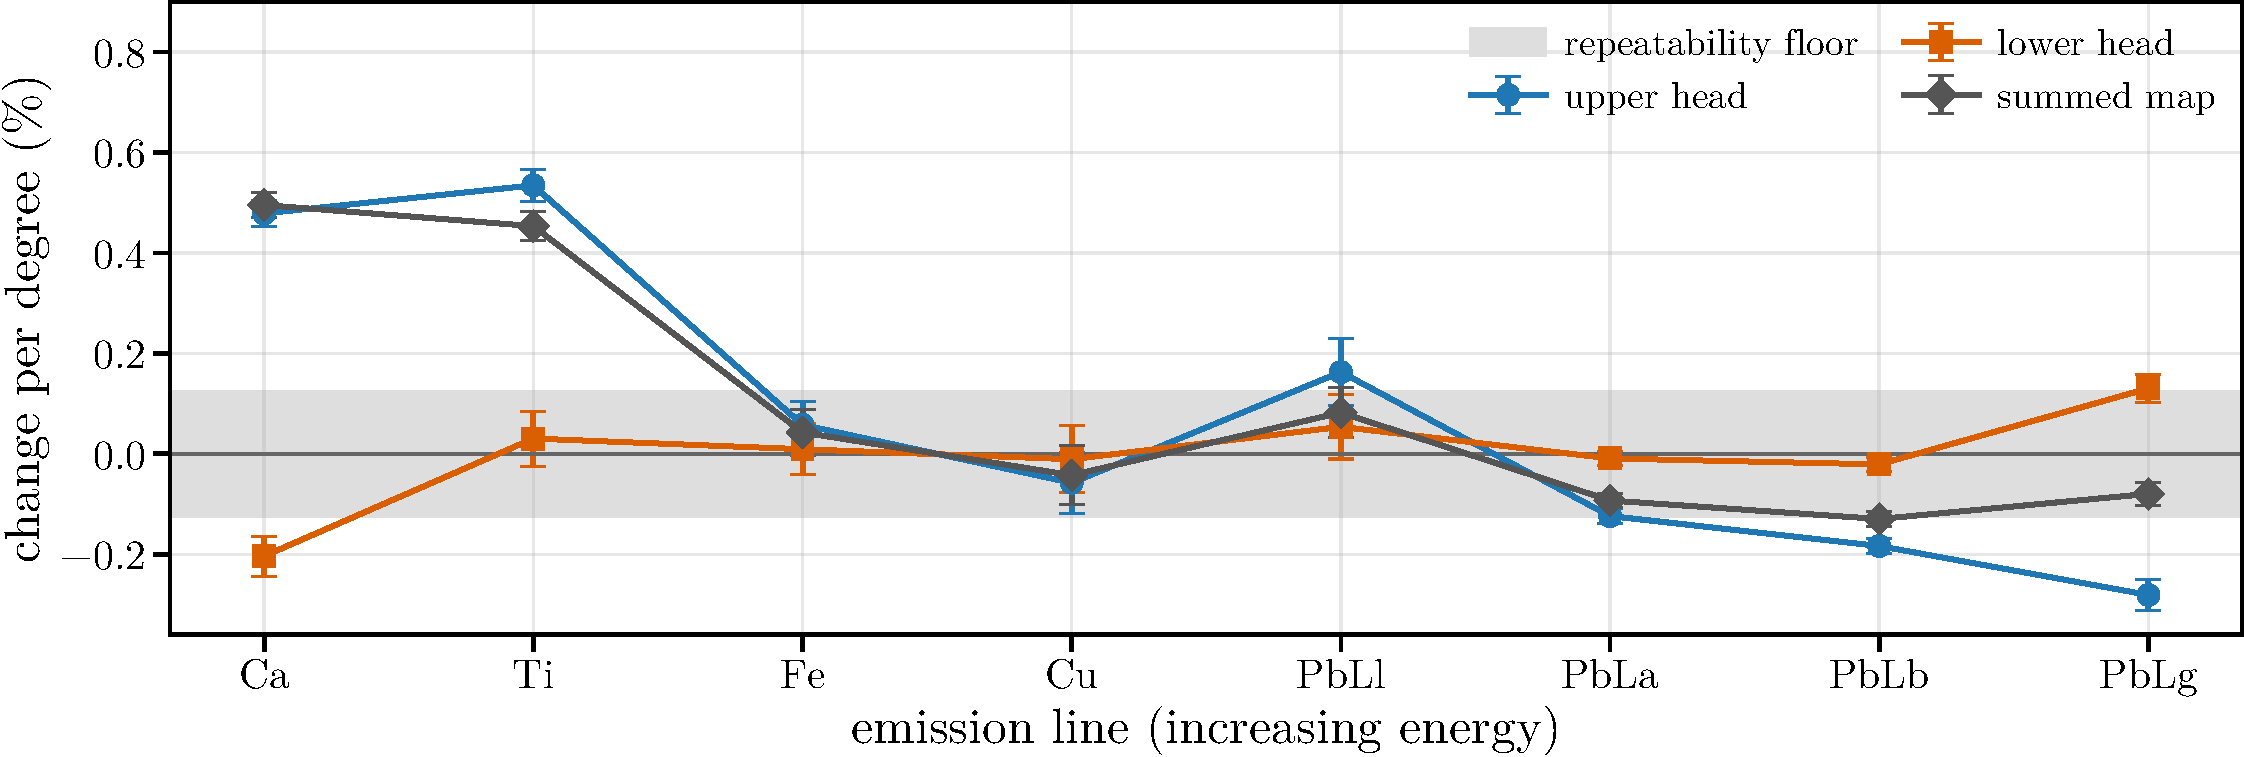
\includegraphics[width=\columnwidth]{figures/block6_positioning_sensitivity.pdf}
\captionof{figure}{The light-element maps are the ones that move; the grey
band is the repeatability floor.}
\end{center}\vspace{0.2cm}
%%%%%%%%%%%%%%%%%%%%%%%%%%%%%%%%%%%%%%%%%%%%%%%%%%%%%%%%%%%%%%%%%%%%%%%%%%%%%%%
%%% END OPTIONAL BLOCK
%%%%%%%%%%%%%%%%%%%%%%%%%%%%%%%%%%%%%%%%%%%%%%%%%%%%%%%%%%%%%%%%%%%%%%%%%%%%%%%

%------------------------------------------------------------------------------
\section*{The scanner characterizes itself from routine scans}

% Take-home box: the one sentence the poster exists for, boxed and a size up,
% where the eye leaves the sheet.
{\setlength{\fboxsep}{0.9cm}\setlength{\fboxrule}{3pt}%
\noindent\fcolorbox{posterblue}{posterblue!6}{%
\parbox{\dimexpr\columnwidth-2\fboxsep-2\fboxrule\relax}{%
\LARGE\bfseries\color{posterblue}%
The difference between a scanner's two detectors, normally summed away, plus
one tilted scan characterizes the instrument for free: detector response,
acquisition geometry, canvas topography, and a learned fusion that beats
summing by 10--18~\% SNR.}}}

\vspace{0.5cm}
Field MA-XRF scanners can be characterized from their own routine scans,
with mounting geometry in the error budget.

%------------------------------------------------------------------------------
\vspace{0.4cm}
% Palace of Science logo beside the sentence that names it.
\noindent
\begin{minipage}[c]{\dimexpr\columnwidth-6.2cm\relax}
{\small
\textbf{Acknowledgements.} The research was partially conducted in the
premises of the Palace of Science, Miodrag Kosti\'{c} Endowment. We thank Ars
Mensurae for instrument access and the scans.
}
\end{minipage}\hfill
\begin{minipage}[c]{5.2cm}

\includegraphics[width=5.2cm]{figures/logo_palata.png}
\end{minipage}

\end{multicols}

\end{document}

%==============================================================================
%  CUT FOR SPACE -- kept here so nothing has to be re-derived.
%==============================================================================
%
%  Per-line ratio table (figures/ratio_table.tex, still generated by
%  scripts/18_poster_figures.py).  The hero figure plots the same numbers.
%
% \vspace{0.3cm}
% \begin{center}
% {\large % generated by scripts/18_poster_figures.py -- do not edit by hand
% source: results/registration/overlap_ratios.csv (script 08)
% tabular* + \extracolsep{\fill}: set to the full column width, so the
% table reads as a block instead of a narrow island.
\begin{tabular*}{\columnwidth}{@{\extracolsep{\fill}} l r r r}
\toprule
\textbf{Line} & \textbf{keV} & $\mathbf{R}$ & \textbf{tilt shift} \\
\midrule
Ca K$\alpha$ & 3.69 & 5.776 & $+9.5$\,\% (24$\sigma$) \\
Ti K$\alpha$ & 4.51 & 2.422 & $+7.9$\,\% (14$\sigma$) \\
Fe K$\alpha$ & 6.40 & 1.206 & $+3.5$\,\% (9$\sigma$) \\
Cu K$\alpha$ & 8.04 & 1.012 & $+2.5$\,\% (5$\sigma$) \\
Pb L$\ell$ & 9.19 & 0.828 & $+4.1$\,\% (6$\sigma$) \\
Pb L$\alpha$ & 10.54 & 0.765 & $+2.2$\,\% (11$\sigma$) \\
Pb L$\beta$ & 12.61 & 0.699 & $+1.8$\,\% (10$\sigma$) \\
Pb L$\gamma$ & 14.77 & 0.630 & $+0.6$\,\% (2$\sigma$) \\
\bottomrule
\end{tabular*}
}
% \captionof{table}{Frontal ratio and tilt shift per line, on the registered
% overlap.}
% \end{center}
% \vspace{0.2cm}
%
%  The two model equations, transcribed from scripts/07_geometry_fit.py
%  (det_ratio and geom_ratio).
%
% \textbf{Stage 1} fits the frontal curve with a scale $k$, a differential
% absorber $d$ in front of the lower head, and silicon thicknesses $t_1$,
% $t_2$ ($t_2$ fixed at 500~$\mu$m), with NIST mass attenuation coefficients
% (Hubbell and Seltzer, NISTIR 5632, 1995):
% \begin{equation}
% R_{\mathrm{det}}(E) = k \;
%   e^{\rho_{\mathrm{Be}} \mu_{\mathrm{Be}}(E) \, d} \;
%   \frac{1 - e^{-\rho_{\mathrm{Si}} \mu_{\mathrm{Si}}(E) \, t_{1}}}
%        {1 - e^{-\rho_{\mathrm{Si}} \mu_{\mathrm{Si}}(E) \, t_{2}}} .
% \end{equation}
%
% \textbf{Stage 2} fits the tilt shift with a thick-sample model in which a
% tilt $\theta$ moves the take-off angles antisymmetrically,
% $\psi_{\pm} = \psi_0 \pm s\theta$, at incidence
% $\varphi = 90^{\circ} - \theta$:
% \begin{equation}
% g(\theta) = \frac{1/\sin\varphi + x/\sin\psi_{-}}
%                  {1/\sin\varphi + x/\sin\psi_{+}} ,
% \qquad x = \left( E/E_c \right)^{-3} ,
% \end{equation}
% giving $\delta(E) = (1+c)\, g(\theta)/g(0) - 1$.
%==============================================================================
